\documentclass[12pt]{article}

\usepackage{amsmath}
\usepackage{amssymb}
\usepackage{amsfonts}
\usepackage{latexsym}
\usepackage{graphicx}

\setlength\topmargin{-1in}
\setlength{\oddsidemargin}{-0.5in}
%\setlength{\evensidemargin}{1.0in}

%\setlength{\parskip}{3pt plus 2pt}
%\setlength{\parindent}{30pt}
%\setlength{\marginparsep}{0.75cm}
%\setlength{\marginparwidth}{2.5cm}
%\setlength{\marginparpush}{1.0cm}
\setlength{\textwidth}{7.5in}
\setlength{\textheight}{10in}


\usepackage{listings}




\newcommand{\pset}[1]{ \mathcal{P}(#1) }


\newcommand{\nats}[0] { \mathbb{N}}
\newcommand{\reals}[0] { \mathbb{R}}
\newcommand{\exreals}[0] {  [-\infty,\infty] }
\newcommand{\eps}[0] {  \epsilon }
\newcommand{\A}[0] { \mathcal{A} }
\newcommand{\B}[0] { \mathcal{B} }
\newcommand{\C}[0] { \mathcal{C} }
\newcommand{\D}[0] { \mathcal{D} }
\newcommand{\E}[0] { \mathcal{E} }
\newcommand{\F}[0] { \mathcal{F} }
\newcommand{\G}[0] { \mathcal{G} }

\newcommand{\IF}[0] { \; \textrm{if} \; }
\newcommand{\THEN}[0] { \; \textrm{then} \; }
\newcommand{\ELSE}[0] { \; \textrm{else} \; }
\newcommand{\AND}[0]{ \; \textrm{ and } \;  }
\newcommand{\OR}[0]{ \; \textrm{ or } \; }

\newcommand{\rimply}[0] { \Rightarrow }
\newcommand{\limply}[0] { \Lefttarrow }
\newcommand{\rlimply}[0] { \Leftrightarrow }
\newcommand{\lrimply}[0] { \Leftrightarrow }

\begin{document}

\begin{flushleft}
Research Documentation - Stochastic Differential Equations Applied to the Linear Wave Equation
Nicholas Maxwell; Dr. Bodmann\\
\end{flushleft}

\begin{flushleft}
\addvspace{5pt} \hrule
\end{flushleft}	



\section*{Part 1 - BM}

\begin{flushleft}
\underline{Construction:}
\end{flushleft}


\begin{flushleft}
$W_t := W(t,\omega)$ a brownian motion. We wish to discretize it in time for numerical purposes, for now we use a regular discretization, so $t_k = j \cdot dt$, then $W_j = W(t_j, \omega)$. We discuss three ways to build $( W_j: j \ge 0 )$
\end{flushleft}

\begin{flushleft}
First we construct a BM directly, by setting $dW_j$ to a standard normal variable, then $W_{j+1} = W_j + \sqrt{dt} \, dW_j$. We test this using the random number generators supplied with the GSL, we pass two uniformly distributed random numbers in $[0,1]$, to the box-muller transfrom to generate two values of $dW$.
\end{flushleft}

\begin{flushleft}
Second we use regular random walks, so $dW_j \in \{-\sqrt{dt} , +\sqrt{dt} \}, P(dW_j = +\sqrt{dt}) = P(dW_j = -\sqrt{dt}) = \frac{1}{2}$, then $W_{t_k} = \sum_{j=1}^{k} \, dW_j$.
\end{flushleft}

\begin{flushleft}
Our third apporach adapts the second. Let $y_j = \{ 1 \IF dW_j = +\sqrt{dt}, 0 \IF dW_j = -\sqrt{dt} \}$, then $dW_j = 2h\, y_j-h$, $W_{t_k} = \sum_{j=0}^{k} \, (2h\, y_j-h) =$ $ -k \cdot h + 2h \cdot \sum_{j=0}^{k} \, y_j$, so this looks like a binomial random variable. Then, seeing as $y_j \in \{ 1,0\}$, with even probability, picking 32 $y_j$s (or whatever the integer size used by the rng) is equivalent to picking a 32 bit integer with uniform distribution over the integer's full scale, which is the output of the GSL's rng, depending on which algorithm is used.
\end{flushleft}


\begin{flushleft}
$\Omega_n = \{ \omega_k: 0 \le k < 2^n, \omega_k = (a_{k,0}, a_{k,1}, ... ,a_{k,n-1}), k = \sum_{j=0}^{n-1} a_{n,j} 2^{-j}, a_{k,j} \in \{ 0,1 \} \}$, $P_n(\omega_k) = 2^{-n}$. $X_n: \Omega_n \rightarrow \reals$, $X_n(\omega_k) = \sum_{j=0}^{n-1} a_{n,j} $. $Y_n(\omega_k) := 2 X_n(\omega_k) - n$. $b(x; n) = P_n ( X_n^{-1}( \{ x \}) ) = \binom{n}{x} 2^{-n} $. $g(x; n) := P_n ( Y_n^{-1}( \{ x \}) ) = P_n ( (2 X_n - n)^{-1}( \{ x \}) ) =  b(\frac{x+n}{2}; n) = \binom{n}{\frac{x+n}{2}} 2^{-n} $. \\ 
Then, it is know that for $E(X_n) = \frac{1}{2} n $, $\sigma_{X_n}^2 = \frac{1}{4} n$, so $E(Y_n) = 0$, $\sigma_{Y_n}^2 = n$, so $\sqrt{dt} \cdot Y_k$ has the right properties for a discretized BM.
\end{flushleft}

\begin{flushleft}
\underline{Implementation:}
\end{flushleft}

\begin{flushleft}
This is the psuedo code for the three methods used. Here $<<$ and $>>$ are left and right bit shifts respectively, and \& is the `and' logic.
\end{flushleft}

\lstset{language=c++ }
\begin{lstlisting}

direct_BM ( n_steps, dt )
{
    dW = alloc( n_steps );
    W = alloc( n_steps )
    
    rng.std_normal_rv( dW, n_steps );
    W[0] = 0;
    
    for ( int j=1; j<n_steps; j++ )
        W[run][j] = W[run][j-1] + dW[j-1]*sqrt(dt);
    
    return W;
}

random_walk_regular ( n_steps, dt )
{
    pool = alloc( n_steps/32 )
    walk = alloc( n_steps )
    W = alloc( n_steps )
    
    for ( k=0; k<n_steps/32; k++)
        pool[k] = rng.gen_int();
    
    walk[0] = 0;
    
    i=0, j=0;
    
    for ( k=1; k<n_steps; k++ )
    {
        if ((pool[j] >> i) & 1)
            walk[k] = walk[k-1]+1;
        else
            walk[k] = walk[k-1]-1;
        
        i++;
        
        if ( i >= 32 )
        {
            i=0;
            j++;
        }
    }
    
    for ( int k=0; k<n_steps; k++ )
        W[k] = sqrt(dt)*walk[k];
    
    return W;
}

random_walk_modified ( n_steps, dt )
{
    pool = alloc( n_steps )
    walk = alloc( n_steps )
    W = alloc( n_steps )
    
    for ( k=0; k<n_steps; k++)
        pool[k] = rng.gen_int();
    
    walk[0] = 0;
    
    for ( int k=1; k<n_steps; k++ )
        walk[k] = walk[k-1] + 2*bitsum( pool[k-1] ) -32;
    
    for ( int k=0; k<n_steps; k++ )
        W[k] = sqrt(dt/32)*walk[k];
    
    return W;
}

bitsum ( x )
{
    sum = 0;
    for ( k=0; k<32; k++)
        sum += (x & (1 << k)) >> k;
    return sum;
}

\end{lstlisting}


\begin{flushleft}
\underline{Results:}
\end{flushleft}



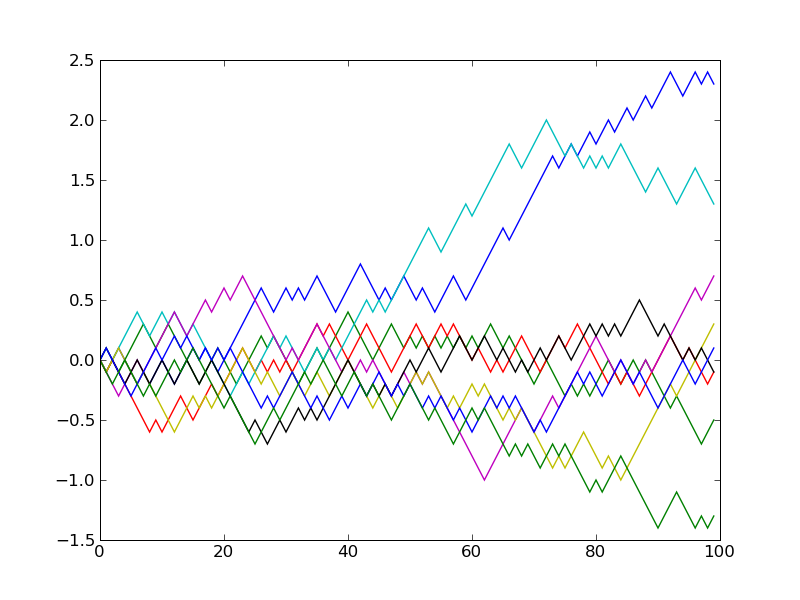
\includegraphics[width=4in]{/workspace/research/SDE/documentation/images/1.png}

Regular random walk, with 100 steps.

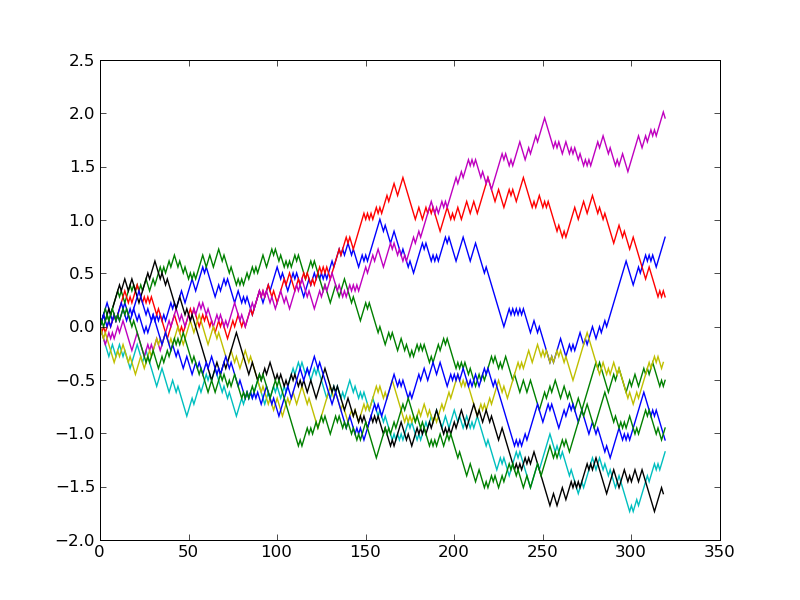
\includegraphics[width=4in]{/workspace/research/SDE/documentation/images/2.png}

Regular random walk, with 320 steps.

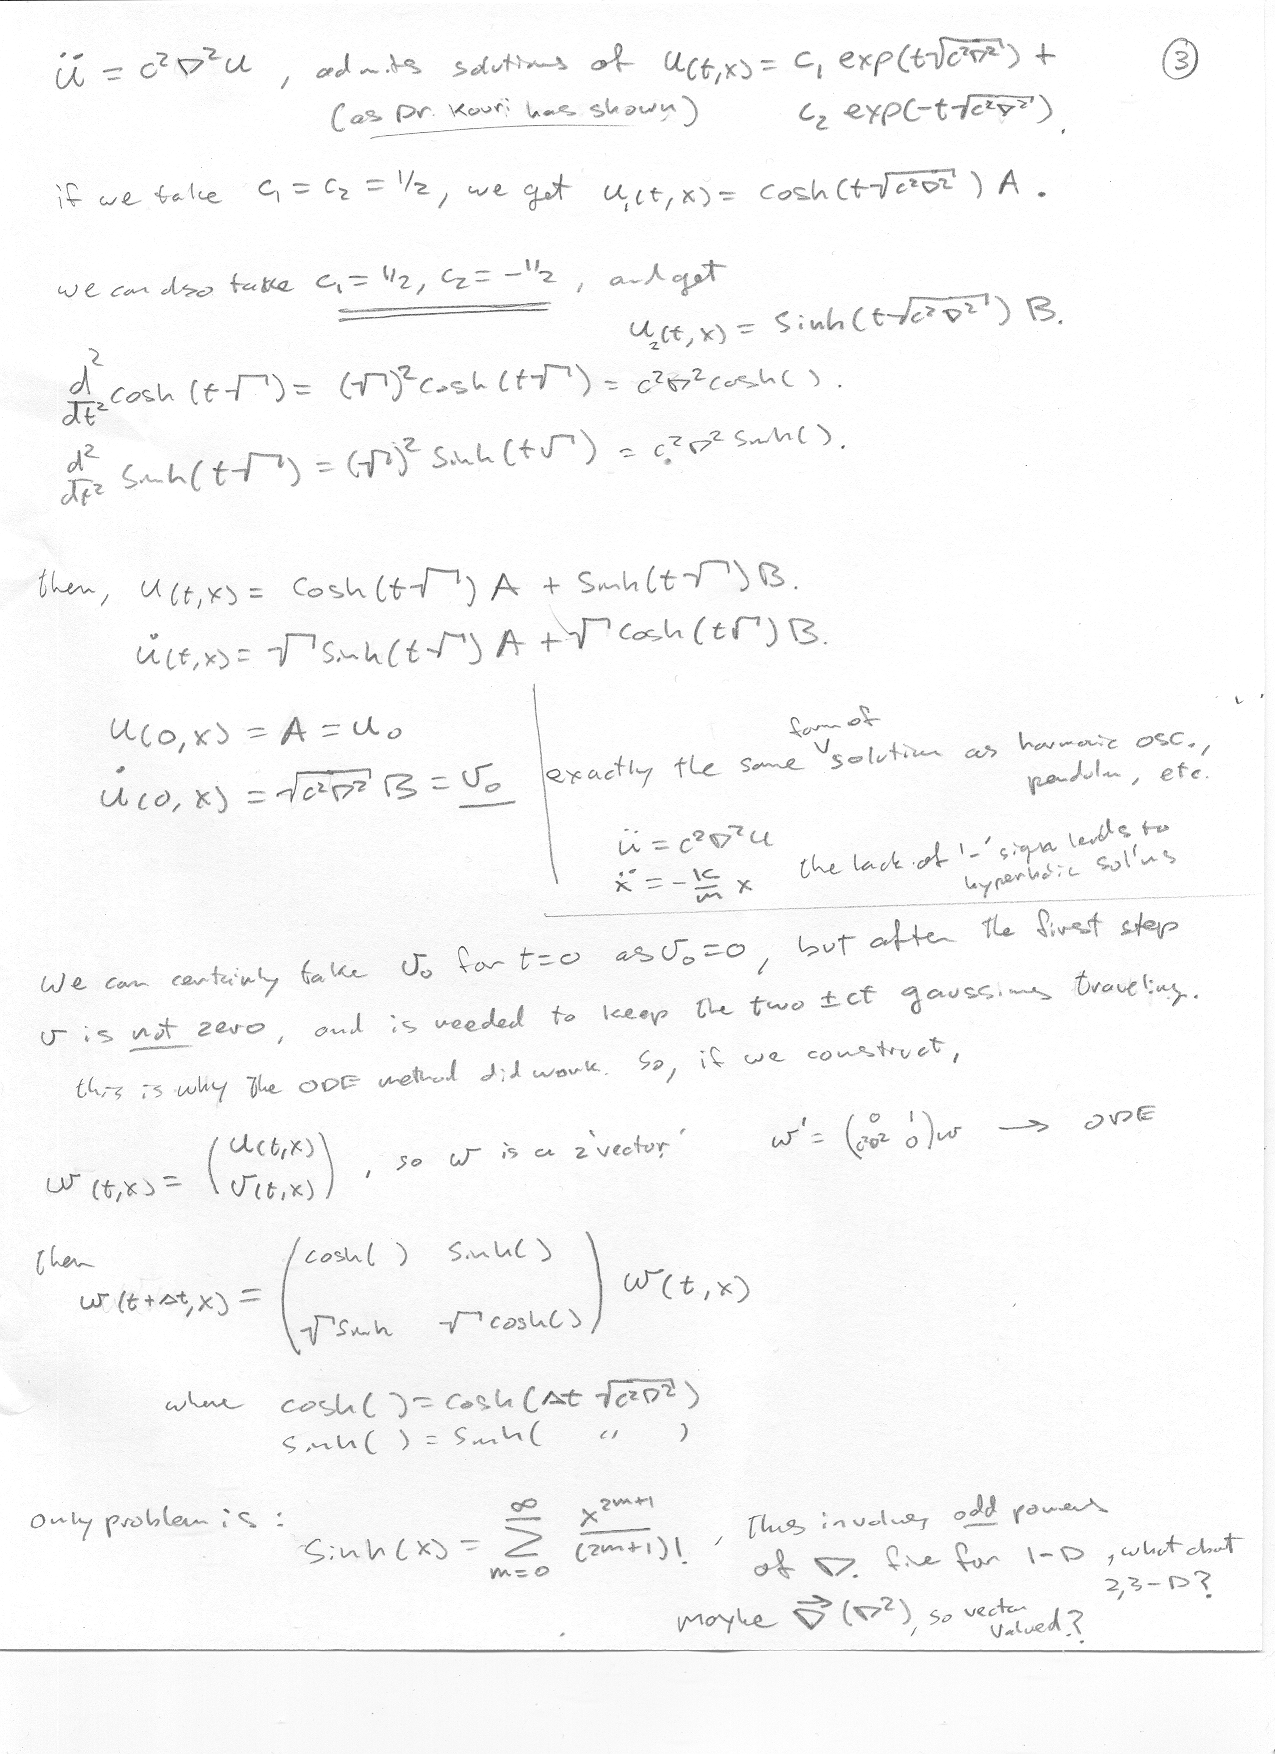
\includegraphics[width=4in]{/workspace/research/SDE/documentation/images/3.png}

Modified random walk, with 100 steps.

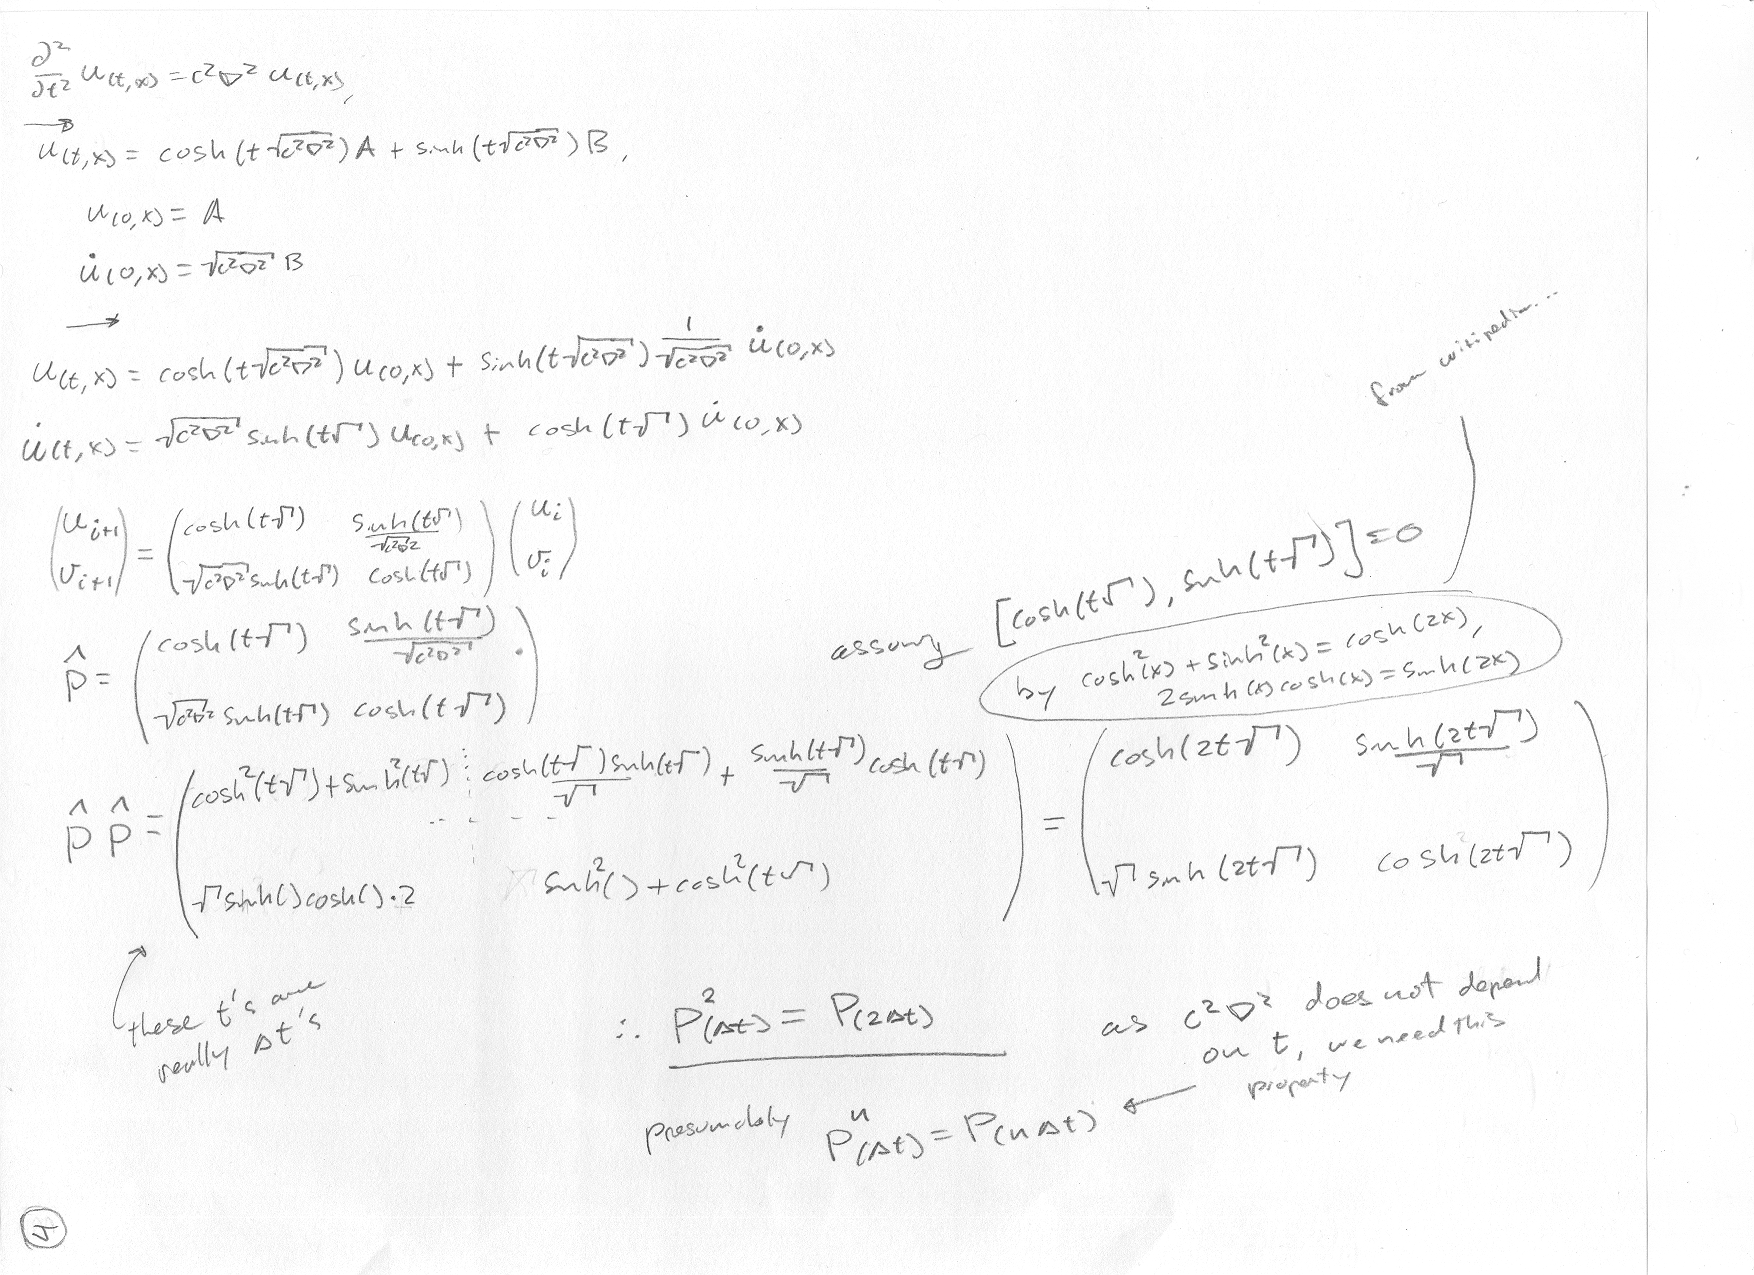
\includegraphics[width=4in]{/workspace/research/SDE/documentation/images/4.png}

Direct construction, with 100 steps.

\begin{flushleft}
Then, to test for the correct mean and standard deviation, 10E5 runs were made at 50 steps per run, at each step the standard deviation and mean were computed for each type of construction. All methods yeilded the correct results ($\pm$ some fractions of a percentage point).
\end{flushleft}

\begin{flushleft}
Then, as an efficiency test, 1E4 runs of 1E3 (32E3 for the regular random walk) steps were performed for each constuction: 3.7 seconds to run for the regular random walk, 0.60 seconds for the modified random walk, and 1.30 seconds for the direct method.
\end{flushleft}


\begin{flushleft}
\underline{Conclusion:}
\end{flushleft}


\begin{flushleft}
The modified random walk method seems to yield similar resutls as the direct method, while being about twice as efficient. It also runs about six times faster than the regular random walk for an equivalent number of steps, this is due primarily due to more efficient code logic (I suspect that the ``bitsum'' function is heavily optimized by the compiler, or even equivalent to a hardware instruction ).
\end{flushleft}


\end{document}


















